\section{Supplementary material}

\paragraph{Simplicial distance and the localizing property of the Laplacian.}
Suppose that $\sigma$ and $\tau$ are $p$-simplices for which $(\nu_0, \nu_1, \dotsc, \nu_d)$ is the shortest sequence of $p$-simplices with the property that $\nu_0=\sigma$, $\nu_d=\tau$, and each $\nu_i$ shares a face or a coface with $\nu_{i-1}$, and a face or a coface with $\nu_{i+1}$. We say that $d$ is the \emph{simplicial distance} between $\sigma$ and $\tau$. Then for all $N<d$, the entry of $L_p^N$ corresponding to $\sigma$ and $\tau$ is $0$, and so the filter does not cause interaction between $c(\sigma)$ and $c(\tau)$. This is analogous to a size-$d$ ordinary CNN layer not distributing information between pixels that are more than $d$ pixels apart. We will refer to $N$ as the \emph{degree} of the convolutional layer, but one may well wish to keep in mind the notion of \emph{size} from traditional CNNs.

\paragraph{Simplicial complexes as the projections of bipartite graphs.}
Given a bipartite graph $X$-$Y$, the simplicial projection on $Y$ is the simplicial complex whose $(k-1)$-simplices are the sets of $k$ vertices in $Y$ that have at least one common neighbor in $X$.
Cochains on the simplicial projection are naturally given by weights on $X$: Given any $(k-1)$-simplex $[y_1,\dots,y_k]$ and its neighboring vertices $\{x_1,\dots,x_j\}\subseteq X$, one can define a $(k-1)$-cochain as $\phi(\{x_1,\dots,x_j\})$, for any function $\phi: \mathcal{P(X)}\to\RR$.
In our coauthorship application, $\phi$ is the sum and the weight of a paper is the number of times it is cited.
See Figure~\ref{fig:bipartite}.

\begin{figure}[htpb]
%\begin{table*}[!t]
\savebox{\tempbox}{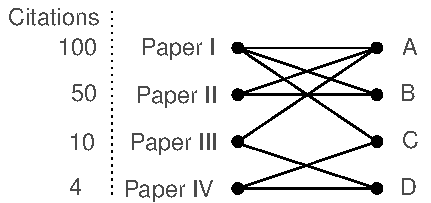
\includegraphics[height=2.3cm]{./figures/bipartite.pdf}}%
\settowidth{\tempwidth}{\usebox{\tempbox}}%
\hfil\begin{minipage}[b]{\tempwidth}%
\raisebox{-\height}{\usebox{\tempbox}}%
%\vspace{-7pt}
\scriptsize{\caption*{(a)}}%
\end{minipage}%
\savebox{\tempbox}{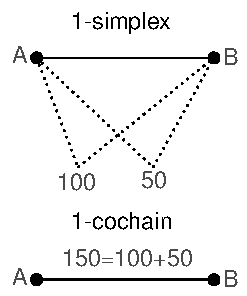
\includegraphics[height=2.5cm]{./figures/cochain.pdf}}%
\settowidth{\tempwidth}{\usebox{\tempbox}}%
\hfil\begin{minipage}[b]{\tempwidth}%
\raisebox{-\height}{\usebox{\tempbox}}%
\scriptsize{\captionof*{figure}{(b)}}%
\end{minipage}%
\vspace{5pt}
%\end{table*}
\savebox{\tempbox}{
\begin{tikzpicture}[font=\scriptsize] % Dirty last minute TikZ with calc cheating and hardcoding.
  \coordinate (b) at (0,0);
  \coordinate (c) at (2.7,0); %($ (b) + (20:2) $);
  \coordinate (a) at (1.35,1.35); %($ (b) + (80:2) $);
  \coordinate (d) at (3.7,0.8); %($ (c) + (30:2) $);

  \draw[twosimp] (a) -- (b) -- (c) -- cycle;
  \draw (a) -- (d) -- (c) -- cycle;
  \fill[color=black] (a) circle (1.5pt);
  \fill[color=black] (b) circle (1.5pt);
  \fill[color=black] (c) circle (1.5pt);
  \fill[color=black] (d) circle (1.5pt);

  \draw (a) -- (b) node [midway,sloped,above] {$150$};
  \draw (a) -- (c) node [midway,sloped,above] {$100$};
  \draw (b) -- (c) node [midway,sloped,below] {$100$};
  \draw (c) -- (d) node [midway,sloped,below] {$4$};
  \draw (a) -- (d) node [midway,sloped,above] {$10$};
  %\node () at ($ (b) + (50:1.15) $) {$100$};
  \node () at (1.3,0.5) {$100$};
  
  \node[anchor=south west] at (a) {$160$};
  \node[anchor=south east] at (a) {$A$};
  
  \node[anchor=north] at (b) {$150$};
  \node[anchor=south] at (b) {$B$};

  \node[anchor=north] at (c) {$104$};
  \node[anchor=south] at (c) {$C$};

  \node[anchor=north] at (d) {$14$};
  \node[anchor=south] at (d) {$D$};
\end{tikzpicture}

}%%
\settowidth{\tempwidth}{\usebox{\tempbox}}%
\hfil\begin{minipage}[b]{\tempwidth}%
\raisebox{-\height}{\usebox{\tempbox}}%
\scriptsize{\captionof*{figure}{(c)}}%
\end{minipage}%
%\end{table*}
\caption{%
    Constructing a simplicial complex and its cochain from a bipartite graph.
    (a)~Paper-author bipartite graph (same data as in Figure~\ref{fig:data2complex}).
    (b)~The $1$-simplex $[A,B]$ is included in the coauthorship complex since authors $A$ and $B$ collaborated.
    The cochain on $[A,B]$ is given by the sum of their common papers' citations.
    (c)~Resulting coauthorship complex with cochains.
}\label{fig:bipartite}
\end{figure}

\begin{table}[htbp]
  \centering
  \scriptsize{
  \begin{tabular}{lrrrrrrrrrrr}
    \toprule
    Dimension   & 0     & 1  & 2     & 3 & 4     & 5 & 6    & 7 & 8   & 9 & 10\\
    \midrule
    CC1 & 352  & 1474  & 3285  & 5019  & 5559  & 4547  & 2732  & 1175  & 343 & 61 & 5\\
    CC2 & 1126 & 5059 & 11840 & 18822 & 21472 & 17896  & 10847 & 4673 & 1357 & 238 & 19\\
    \bottomrule
  \end{tabular}}
  \vspace{2pt}
  \caption{%
  Number of simplices of the two coauthorship complexes sampled from Semantic Scholar.
  } \label{table:Simplices-coauthor}
\end{table}

\paragraph{Sampling papers.}
From the Semantic Scholar Open Research Corpus~\cite{ammar18NAACL}, we excluded papers with fewer than $5$ citations or more than $10$ authors.
To sample a CC, we sampled $80$ papers (corresponding to \mdeff{top-dimensional/maximal, what's the term?} simplices in the CC) by performing a random walk (of length $80$) on the graph whose vertices represent papers and edges connect papers sharing at least one author.

\paragraph{Mean accuracy and absolute error.}
A missing value is considered to be correctly imputed if the imputed value differs by at most $10\%$ from the true value.
The \emph{accuracy} is the percentage of missing values that has been correctly imputed and the \emph{absolute error} is the magnitude of the difference between the imputed and true value.
For each rate of missing values, we compute the \emph{mean accuracy} $\pm$ standard deviation over 5 samples with randomly damaged portions.
